\documentclass[11pt,a4paper]{article}

\usepackage[utf8]{inputenc}
\usepackage{geometry}
\geometry{a4paper, margin=1in}
\usepackage{graphicx}
\usepackage{amsmath, amssymb}
\usepackage{hyperref}
\usepackage{booktabs}
\usepackage{enumitem}
\usepackage{caption}
\usepackage{subcaption}
\usepackage{multirow}

\title{A Multi-Agent, Local-First Edge AI Architecture for Autonomous Residential Energy Optimisation Under Dynamic Tariffs}
\author{Somayajula Aryan}
\date{May 2026}

\begin{document}

% --- TITLE PAGE ---
\maketitle
\thispagestyle{empty}
\newpage

% --- ABSTRACT PAGE ---
\begin{abstract}
Residential energy systems remain inefficient despite the proliferation of smart home technologies, largely due to limitations in existing Home Energy Management Systems (HEMS). These limitations include heavy cloud dependence, constrained learning capabilities, and poor integration with dynamic energy pricing structures. While recent advances in edge artificial intelligence (AI) and reinforcement learning (RL) offer significant potential for autonomous optimisation, existing approaches remain challenging to deploy in real-world residential environments due to cold-start issues, sensing constraints, and long-term model degradation. This paper presents a multi-agent, local-first edge AI architecture for autonomous residential energy optimisation under dynamic tariffs. The proposed system decomposes intelligence into three cooperative agents: (i) an Energy Agent for tariff-aware load scheduling using time-series forecasting and optimisation; (ii) an Automation Agent that models occupant behaviour using RL and probabilistic inference; and (iii) a System Agent that ensures long-term robustness through resource management and adaptive model maintenance. All computation is executed locally on edge hardware, enabling real-time control, preserving occupant privacy, and ensuring resilience against connectivity failures. We implement a digital twin simulation environment and evaluate the architecture across four tariff scenarios using 20 Monte Carlo trials each. Results demonstrate mean cost reductions of \textbf{9.2--12.8\%} relative to a no-optimisation baseline, with the hybrid multi-agent system achieving competitive performance against static rule-based controllers while offering superior adaptability on volatile tariffs.
\end{abstract}
\newpage

% --- TABLE OF CONTENTS PAGE ---
\tableofcontents
\newpage

% --- MAIN CONTENT START ---
\section{Introduction}

\subsection{Background and Motivation}
Residential buildings account for a substantial share of global energy consumption, with heating, cooling, and appliance usage constituting the primary load components. Despite the increasing availability of smart home technologies, most residential environments remain reactive rather than intelligent, relying heavily on fixed schedules, manual control, or simple rule-based automation. As electricity markets transition toward dynamic pricing models, including time-of-use (ToU) and real-time tariffs, the economic and operational limitations of static control strategies become increasingly evident.

Current smart home platforms are predominantly cloud-centric, mediating sensing, decision-making, and control through remote infrastructure. While this paradigm enables scalable data aggregation, it introduces several critical vulnerabilities: (i) privacy concerns arising from the continuous transmission of behavioural data; (ii) latency constraints that hinder real-time control applications; and (iii) a strict reliance on network connectivity, which diminishes overall system robustness. These limitations are particularly acute in residential environments, where reliability, responsiveness, and user trust are paramount \cite{zipperer2013electric}.

Simultaneously, advances in machine learning (ML), particularly reinforcement learning (RL) and time-series forecasting, have demonstrated strong potential for demand-side energy optimisation. Prior studies report energy savings in the range of 10\% to 30\% utilizing learning-based approaches \cite{vazquez2019reinforcement, wang2020reinforcement}. However, these methods are typically evaluated in highly controlled environments, assume the presence of extensive sensing infrastructure, or fail to account for real-world deployment constraints such as hardware limitations, occupant variability, and long-term system maintenance.

\subsection{Research Gap}
Despite significant progress across academia and industry, a persistent gap remains between theoretically optimal energy management approaches and systems that can be practically deployed in residential settings. Existing solutions largely fail to simultaneously address the following challenges:

\begin{itemize}[leftmargin=*]
    \item \textbf{Local-First Intelligence:} Most systems rely on cloud-based computation, with limited exploration of fully on-device learning and control.
    \item \textbf{Cold-Start and User Acceptance:} Learning-based systems often exhibit poor initial performance, leading to reduced user trust and subsequent disengagement.
    \item \textbf{Scalable Sensing:} Appliance-level monitoring typically requires intrusive hardware, fundamentally limiting scalability and broad adoption.
    \item \textbf{Integrated Optimisation:} Energy cost, occupant comfort, and system constraints are rarely jointly optimised within a unified framework.
    \item \textbf{Model Lifecycle Management:} Very few studies address long-term model degradation, concept drift, and adaptive retraining over multi-year deployments.
\end{itemize}

This fragmentation results in systems that are either theoretically sophisticated but impractical for real-world use, or highly deployable but severely limited in intelligence and adaptability.

\subsection{Proposed Approach}
To address these limitations, this paper proposes a multi-agent, local-first edge AI architecture designed for autonomous residential energy optimisation under dynamic tariff conditions. The system decomposes intelligence into three cooperative agents, each responsible for a distinct functional domain.

The \textit{Energy Agent} performs tariff-aware optimisation by combining time-series forecasting methods---such as gradient boosting and recurrent neural networks---with scheduling algorithms to shift loads toward low-cost periods. The \textit{Automation Agent} models occupant behaviour using RL and probabilistic inference, enabling the adaptive and personalised control of devices based on learned routines. Finally, the \textit{System Agent} monitors computational resources and model performance, enabling dynamic resource allocation and lifecycle-aware model maintenance.

A key design feature of the proposed system is the utilization of a hybrid optimisation framework, wherein rule-based constraints guarantee safety and reliability, while learning-based methods provide adaptability and long-term optimisation. This hybrid approach effectively mitigates cold-start issues and ensures stable operation during the critical early phases of deployment. Furthermore, the system incorporates non-intrusive load monitoring (NILM) to achieve appliance-level intelligence without necessitating additional hardware instrumentation \cite{kelly2015neural}.

\subsection{Contributions and Paper Structure}
The primary contributions of this paper are threefold:
\begin{enumerate}[label=\textbf{\arabic*.}]
    \item The introduction of a novel multi-agent, local-first architecture that integrates behavioural learning, tariff-aware optimisation, and system self-management within a unified edge-based framework.
    \item The proposal of a hybrid optimisation approach that combines reinforcement learning, time-series forecasting, and rule-based constraints to effectively address real-world deployment challenges, including cold-start phenomena and system stability.
    \item The empirical validation of this architecture via a reproducible digital twin simulation, demonstrating 9--13\% cost reductions across realistic tariff scenarios with rigorous Monte Carlo statistics.
\end{enumerate}

The remainder of this paper is structured as follows. Section II reviews related work in HEMS, edge AI, and NILM. Section III describes the proposed system architecture. Section IV details the intelligence modules and optimisation framework. Section V presents dynamic tariff integration. Section VI discusses privacy and security considerations. Section VII outlines the evaluation methodology. Section VIII presents empirical results. Section IX examines challenges and limitations. Section X analyses differentiation from existing systems. Section XI discusses future research directions, and Section XII concludes the paper.

\section{Related Work}
\subsection{Home Energy Management Systems (HEMS)}

Home Energy Management Systems (HEMS) have been widely studied as a means to improve residential energy efficiency and enable demand-side management. Early HEMS solutions primarily relied on rule-based control strategies, where predefined schedules and user-defined preferences dictated device operation. While these approaches are simple and interpretable, they lack adaptability to changing user behaviour and dynamic energy pricing \cite{beaudin2015home}.

More recent systems incorporate optimisation-based methods, including linear programming and heuristic scheduling, to minimise energy costs under time-of-use tariffs. However, these approaches often assume perfect knowledge of future demand and do not account for uncertainty in occupant behaviour or environmental conditions. Furthermore, many commercial HEMS platforms, such as smart thermostats and voice-controlled ecosystems, provide limited optimisation capabilities and primarily focus on convenience rather than autonomous energy management \cite{zipperer2013electric}.

\subsection{Machine Learning for Energy Optimisation}

Machine learning techniques, particularly reinforcement learning (RL), have gained attention for their ability to learn adaptive control policies in dynamic environments. RL-based approaches have been applied to HVAC control, appliance scheduling, and demand response, demonstrating significant potential for reducing energy consumption and costs \cite{vazquez2019reinforcement}.

Despite these advances, several limitations persist. First, RL methods typically require extensive training data and exploration, leading to poor performance during initial deployment (i.e., the cold-start problem). Second, many studies evaluate RL models in simulated environments, which may not capture the variability and unpredictability of real-world residential settings. Third, pure RL approaches often lack safety guarantees, making them unsuitable for direct deployment without additional constraints \cite{wang2020reinforcement}.

To address these issues, hybrid approaches combining RL with rule-based control or supervised learning have been proposed. Time-series forecasting methods, including gradient boosting machines (GBM) and recurrent neural networks (RNNs), are commonly used to predict energy demand or price signals. However, existing work rarely integrates forecasting, behavioural learning, and control into a unified framework.

\subsection{Edge AI and Local-First Architectures}

The increasing availability of low-cost edge computing platforms has enabled the deployment of machine learning models directly within residential environments. Edge AI offers several advantages, including reduced latency, improved privacy, and resilience to connectivity failures \cite{shi2016edge, zhou2019edge}. Recent studies have explored on-device inference for smart home applications, such as occupancy detection and anomaly detection.

However, most existing systems adopt a hybrid architecture where data is partially processed locally but relies on cloud infrastructure for training, coordination, or long-term storage. Fully local-first architectures, where sensing, learning, and control are performed entirely on-device, remain underexplored. Additionally, the resource constraints of edge hardware introduce challenges in model selection, computational efficiency, and system scalability \cite{zhou2019edge}.

\subsection{Non-Intrusive Load Monitoring (NILM)}

Non-Intrusive Load Monitoring (NILM) aims to disaggregate aggregate household energy consumption into individual appliance-level usage without requiring dedicated sensors. NILM has been extensively studied using techniques ranging from hidden Markov models to deep learning architectures \cite{hart1992nonintrusive, kelly2015neural}.

While NILM offers a promising pathway for scalable appliance-level intelligence, its real-world performance remains inconsistent, particularly in environments with multiple similar appliances or overlapping usage patterns. Many existing approaches rely on high-frequency data or extensive training datasets, limiting their applicability in low-cost residential deployments. Moreover, NILM is rarely integrated into closed-loop control systems, where disaggregated insights directly inform optimisation decisions.

\subsection{Limitations of Existing Systems}

Across the literature, several recurring limitations can be identified. First, there is a strong reliance on cloud-based architectures, which raises concerns related to privacy, latency, and reliability. Second, learning-based approaches often suffer from cold-start issues and lack mechanisms for stable deployment in real-world environments. Third, most systems treat energy optimisation, behavioural modelling, and system management as separate problems rather than components of a unified architecture.

Finally, long-term system performance remains an underexplored area. Very few studies address model drift, adaptive retraining, or lifecycle management in residential energy systems, despite the fact that occupant behaviour and environmental conditions evolve over time.\\
\textbf{Security and trust in edge systems:} While cloud-based architectures raise privacy concerns, fully local systems introduce new security challenges, including device-level vulnerabilities, insecure communication between components, and lack of standardised authentication mechanisms. Existing HEMS literature provides limited discussion on secure on-device coordination, encryption, and access control in edge AI deployments.

\subsection{Positioning of This Work}

This paper addresses the above limitations by proposing a unified, multi-agent architecture that integrates energy optimisation, behavioural learning, and system-level management within a local-first framework. Unlike prior work, the proposed system explicitly incorporates:

\begin{itemize}
    \item A hybrid optimisation approach combining reinforcement learning, forecasting, and rule-based constraints to ensure both adaptability and stability.
    \item A fully local-first design, where all sensing, learning, and control are executed on edge hardware.
    \item The integration of NILM as a zero-hardware sensing layer within a closed-loop optimisation system.
    \item A lifecycle-aware framework that addresses long-term model drift and system adaptation.
\end{itemize}

By unifying these components, the proposed approach bridges the gap between theoretical optimisation methods and deployable residential energy systems. The proposed system also incorporates secure communication and authentication mechanisms within the edge environment, addressing an often-overlooked challenge in local-first residential energy systems.

\section{System Architecture}

\subsection{Design Principles}

The proposed system is designed based on three core principles: (i) \textit{local-first intelligence}, where sensing, learning, and control are executed entirely on edge hardware; (ii) \textit{modular multi-agent decomposition}, enabling scalable and interpretable system design; and (iii) \textit{robustness and security}, ensuring reliable operation under real-world constraints.

The shift toward edge-based architectures is motivated by increasing concerns around privacy, latency, and bandwidth usage in cloud-centric IoT systems \cite{zhou2019edge, lin2017survey}. By performing computation locally, the system reduces dependence on external infrastructure while enabling real-time responsiveness and improved data sovereignty.

\subsection{Multi-Agent System Design}

The architecture decomposes system intelligence into three cooperative agents: the Energy Agent, the Automation Agent, and the System Agent. This decomposition allows separation of forecasting, control, and lifecycle management, improving scalability and maintainability.

\subsubsection{Energy Agent}

The Energy Agent is responsible for tariff-aware optimisation of residential energy consumption. It integrates external signals such as dynamic pricing, weather forecasts, and historical usage data to generate predictive control strategies.

Time-series forecasting models, including gradient boosting machines (GBM) and recurrent neural networks (RNNs), are used to estimate short-term demand and price trends \cite{hong2016probabilistic}. These predictions are incorporated into a scheduling framework that shifts flexible loads toward low-cost periods, consistent with demand response strategies explored in prior work \cite{paterakis2017overview}.

\subsubsection{Automation Agent}

The Automation Agent models occupant behaviour and device usage patterns through reinforcement learning. The agent observes system states, including NILM-derived appliance activity, environmental conditions, and historical actions, and learns policies that optimise long-term reward functions.

Reinforcement learning has been widely applied in residential energy systems for HVAC control and load scheduling \cite{wang2020reinforcement}. However, to address known challenges such as instability and unsafe exploration, the proposed system employs a hybrid approach where RL policies are constrained by rule-based safety mechanisms \cite{garcia2015comprehensive}. This ensures that control actions remain within acceptable operational and comfort boundaries.

\subsubsection{System Agent}

The System Agent is responsible for system-level coordination, resource management, and lifecycle-aware adaptation. It continuously monitors model performance, computational load, and system health, enabling dynamic allocation of resources across agents.

In addition, the System Agent implements mechanisms for detecting model drift and triggering retraining or adaptation. Long-term model degradation remains an underexplored problem in residential energy systems \cite{dincecco2020transfer}, motivating the need for lifecycle-aware architectures.

\subsection{Data Flow and Local Communication}

The system operates through a local data pipeline where sensor inputs, model outputs, and control signals are exchanged between agents in real time. Communication is implemented using lightweight messaging protocols such as MQTT, which are commonly used in IoT systems due to their low overhead and scalability \cite{naik2017choice}.

Direct hardware interfacing is achieved through local input/output mechanisms, enabling control of appliances, sensors, and actuators without cloud mediation. This design ensures low-latency actuation and resilience to network disruptions.

\subsection{Integration of NILM as a Sensing Layer}

Non-Intrusive Load Monitoring (NILM) is integrated as a core sensing component, enabling appliance-level visibility using aggregate energy data. NILM has been widely studied as a cost-effective alternative to intrusive sub-metering \cite{ruano2019nilm}.

However, prior work highlights significant challenges in real-world deployment, including reduced accuracy in multi-appliance environments and sensitivity to data sparsity \cite{tang2023nilm}. To address these limitations, the system treats NILM outputs as probabilistic signals rather than deterministic ground truth, allowing downstream agents to account for uncertainty in decision-making.

\subsection{Security and Trust Model}

Given the local-first architecture, security is addressed through a combination of encrypted communication, authentication, and system isolation. All inter-agent communication is secured using transport-layer encryption (e.g., TLS), ensuring data confidentiality and integrity within the local network \cite{kothmayr2013dtls}.

Authentication is enforced using token-based mechanisms to verify the identity of system components and prevent unauthorised access. Additionally, modular separation between agents provides logical isolation, reducing the risk of cascading failures or system-wide compromise.

This approach addresses a critical gap in existing HEMS research, where security considerations in fully local AI systems remain underexplored.

\subsection{Hybrid Intelligence Framework}

A defining feature of the proposed architecture is the integration of multiple learning paradigms within a unified framework. Rule-based control provides safety and interpretability, particularly during early deployment phases. Forecasting models enable anticipatory decision-making, while reinforcement learning provides long-term adaptability.

Hybrid approaches have been shown to improve stability and performance in real-world control systems \cite{mason2019reinforcement}. By combining these methods, the proposed system mitigates the limitations of individual techniques while enabling scalable and robust residential energy optimisation.

\section{Intelligence Modules and Optimisation Framework}

\subsection{Problem Formulation}

The objective of the proposed system is to optimise residential energy consumption under dynamic pricing while maintaining occupant comfort and respecting device-level constraints. This is formulated as a multi-objective optimisation problem.

Let the time horizon be discretised into intervals $t \in \{1, 2, ..., T\}$. At each time step, the system observes the state $s_t$ and selects an action $a_t$.

The optimisation objective is defined as:

$$
\min_{\pi} \ \mathbb{E} \left[ \sum_{t=1}^{T} \left( C_t(s_t, a_t) + \lambda \cdot D_t(s_t, a_t) \right) \right]
$$

where:
\begin{itemize}
    \item $C_t$ represents energy cost under dynamic tariffs,
    \item $D_t$ represents discomfort or deviation from user preferences,
    \item $\lambda$ is a weighting factor controlling the trade-off between cost and comfort,
    \item $\pi$ is the control policy.
\end{itemize}

\subsection{System State Representation}

The system state $s_t$ is defined as a multi-dimensional vector:

$$
s_t = \{ L_t, P_t, O_t, E_t, N_t \}
$$

where:
\begin{itemize}
    \item $L_t$: aggregate load and historical consumption,
    \item $P_t$: dynamic tariff and price forecasts,
    \item $O_t$: occupancy and behavioural context,
    \item $E_t$: environmental variables (e.g., temperature, weather),
    \item $N_t$: NILM-derived appliance-level activity.
\end{itemize}

NILM outputs are treated as probabilistic estimates due to known uncertainty in multi-appliance environments \cite{tang2023nilm}.

\subsection{Action Space}

The action space $a_t$ consists of control decisions over devices:

$$
a_t = \{ u^{HVAC}_t, u^{appliance}_t, u^{storage}_t \}
$$

where:
\begin{itemize}
    \item $u^{HVAC}_t$: thermostat setpoint adjustments,
    \item $u^{appliance}_t$: scheduling or deferral of controllable loads,
    \item $u^{storage}_t$: battery charging/discharging decisions (if available).
\end{itemize}

All actions are subject to operational constraints:

$$
a_t \in \mathcal{A}_{safe}
$$

where $\mathcal{A}_{safe}$ encodes device limits, safety rules, and comfort bounds.

\subsection{Energy Agent: Forecasting and Scheduling}

The Energy Agent performs short-term forecasting and scheduling using supervised learning models.

Given historical data $\{L_{t-k}, ..., L_t\}$ and external features, the forecasting model predicts future demand:

$$
\hat{L}_{t+1:t+H} = f_{\theta}(L_{t-k:t}, P_{t:t+H}, E_{t:t+H})
$$

where $f_{\theta}$ represents a trained model such as:
\begin{itemize}
    \item Gradient Boosting Machines (GBM),
    \item Long Short-Term Memory (LSTM) networks.
\end{itemize}

These forecasts are combined with tariff signals to generate a baseline schedule:

$$
\min_{u} \sum_{t=1}^{T} P_t \cdot u_t
$$

subject to:
\begin{itemize}
    \item device constraints,
    \item user-defined preferences,
    \item predicted demand requirements.
\end{itemize}

\subsection{Automation Agent: Reinforcement Learning Control}

The Automation Agent refines control decisions using reinforcement learning.

The environment is modelled as a Markov Decision Process (MDP):

$$
\mathcal{M} = (\mathcal{S}, \mathcal{A}, \mathcal{P}, \mathcal{R})
$$

where:
\begin{itemize}
    \item $\mathcal{S}$: state space,
    \item $\mathcal{A}$: action space,
    \item $\mathcal{P}$: transition dynamics,
    \item $\mathcal{R}$: reward function.
\end{itemize}

The reward function is defined as:

$$
R_t = - \left( C_t + \lambda D_t \right)
$$

The RL agent learns a policy $\pi(a_t | s_t)$ that maximises expected cumulative reward:

$$
\max_{\pi} \ \mathbb{E} \left[ \sum_{t=1}^{T} \gamma^t R_t \right]
$$

where $\gamma$ is the discount factor.

To ensure safe deployment, the RL policy is constrained by rule-based filters:

$$
a_t = \Pi_{safe}(\pi(s_t))
$$

where $\Pi_{safe}$ projects actions onto the safe action set.

This hybrid formulation mitigates instability and unsafe exploration commonly observed in pure RL systems \cite{garcia2015comprehensive}.

\subsection{System Agent: Lifecycle and Drift Management}

The System Agent monitors model performance and detects drift over time.

Let $\epsilon_t$ denote prediction error:

$$
\epsilon_t = |L_t - \hat{L}_t|
$$

Drift is detected when:

$$
\mathbb{E}[\epsilon_t] > \delta
$$

where $\delta$ is a predefined threshold.

Upon drift detection, the system triggers:
\begin{itemize}
    \item model retraining,
    \item parameter adaptation,
    \item or fallback to rule-based control.
\end{itemize}

This addresses the lack of lifecycle-aware strategies in existing HEMS research \cite{dincecco2020transfer}.

\subsection{Hybrid Optimisation Strategy}

The overall control strategy combines three layers:

\begin{enumerate}
    \item Rule-based baseline for safety and cold-start,
    \item Forecast-driven optimisation for anticipatory scheduling,
    \item RL-based adaptation for long-term improvement.
\end{enumerate}

The final control action is:

$$
a_t = \Pi_{safe} \left( \alpha \cdot a_t^{RL} + (1-\alpha) \cdot a_t^{forecast} \right)
$$

where $\alpha$ is adaptively tuned based on system confidence.

\subsection{Data Pipeline and Edge Deployment}

The system operates on continuous data streams:

\begin{itemize}
    \item Smart meter readings (aggregate load),
    \item Tariff data (e.g., half-hourly pricing),
    \item Environmental data (weather APIs),
    \item Device states and control signals,
    \item NILM-inferred appliance usage.
\end{itemize}

Data are processed locally using a streaming pipeline. Model inference is executed on edge hardware, while training is performed incrementally or during low-load periods.

To accommodate hardware constraints, lightweight models and batching strategies are employed, ensuring real-time performance within resource limits.


\section{Dynamic Tariff Integration and Economic Optimisation}

\subsection{The Dynamic Pricing Model}

As global energy grids modernise, residential electricity pricing is increasingly shifting away from flat rates and toward dynamic tariff structures. In these models, the price of electricity fluctuates based on real-time supply and demand conditions. If we let $P_t$ denote the electricity price at time step $t$, we can represent a dynamic tariff as:

$$P_t=P^{base}+\Delta P_t$$

where:
\begin{itemize}
    \item $P^{base}$ is the standard baseline tariff,
    \item $\Delta P_t$ represents time-varying adjustments driven by market conditions.
\end{itemize}

In real-world deployments, this $\Delta P_t$ value is often derived from wholesale market signals, such as the half-hourly pricing models seen in innovative utility offerings like the Octopus Agile tariff. By tapping into these signals, the system can capitalise on periods of excess renewable generation when energy is cheapest (or even negatively priced) \cite{mohsenian2010autonomous}.

\subsection{Navigating Forecast Uncertainty}

Because the future is never perfectly predictable, the system cannot rely solely on current prices; it must anticipate them. We incorporate short-term tariff forecasting to look ahead:

$$\hat{P}_{t+1:t+H}=g_{\phi}(P_{t-k:t}, M_t)$$

where $g_{\phi}$ is a forecasting model (such as a Gradient Boosting Machine) and $M_t$ represents external market indicators.

Crucially, forecast uncertainty is modelled using confidence intervals ($\hat{P}_t\pm\sigma_t$). Rather than assuming a prediction is flawlessly accurate, this allows the system to make risk-aware decisions---avoiding high-stakes gambles when market volatility is high.

\subsection{Integrating Cost into the Agent's Mandate}

To optimise for economic efficiency, we must first define the physical cost of energy at any given time. This is simply the product of the dynamic price and the energy consumed:

$$C_t=P_t \cdot E_t$$

where $E_t$ is the energy consumption resulting from the system's chosen action $a_t$. By substituting this into our primary optimisation objective, we give the system a clear financial mandate:

$$\min \sum_{t=1}^{T} P_t \cdot E_t + \lambda D_t$$

This formulation ensures the agent actively balances the raw financial cost of energy consumption against the user's comfort ($D_t$), guided by the sensitivity weight ($\lambda$).

\subsection{Demand-Side Flexibility and Load Shifting}

One of the most powerful ways the system saves money is by treating household appliances as flexible assets. By shifting controllable loads across the day, the system minimises costs:

$$\min \sum_{t=1}^{T} P_t \cdot u_t$$

subject to the constraint that the task must actually be completed within an acceptable timeframe:

$$\sum_{t \in \mathcal{T}_i} u_t=E_i^{req}$$

where $\mathcal{T}_i$ is the allowable time window for appliance $i$, and $E_i^{req}$ is the total energy required to complete the task. In practical terms, this means the system can automatically defer high-consumption chores---like running a dishwasher or charging an electric vehicle---until the grid signals an abundance of cheap energy, all without the homeowner needing to lift a finger.

\subsection{Real-Time Responsiveness}

Beyond long-term scheduling, the edge architecture allows the system to react instantly to sudden price spikes. These real-time control adjustments include:
\begin{itemize}
    \item Modulating HVAC setpoints by a few degrees during peak price events,
    \item Initiating temporary load shedding for non-essential devices,
    \item Discharging a home battery to offset grid consumption.
\end{itemize}

To teach the Reinforcement Learning (RL) agent to do this naturally, the reward function directly incorporates tariff sensitivity:

$$R_t=-\left( P_t \cdot E_t + \lambda D_t \right)$$

This forces the agent to learn policies that inherently respect the ebb and flow of dynamic pricing.

\subsection{Risk-Aware Optimisation}

Wholesale energy markets can be highly volatile. To protect the homeowner from sudden price shocks, the system employs a risk-sensitive optimisation strategy:

$$\min \ \mathbb{E}[C_t] + \beta \cdot \text{Var}(C_t)$$

Here, $\beta$ acts as a risk-aversion dial. This mathematical safeguard ensures that the system avoids "optimal" schedules that are too fragile or overly dependent on highly uncertain price forecasts.

\subsection{Local-First API Integration}

To fuel these decisions, the system interfaces with external tariff providers (such as utility APIs or regional grid operators). However, to preserve our strict local-first architecture, tariff data is fetched periodically and cached locally on the edge device. If the home loses its internet connection, the system simply falls back on its latest cached forecasts and historical trends, ensuring uninterrupted economic optimisation.

\subsection{Personalisation: Cost vs. Comfort}

Every household is unique. Some users are highly motivated to slash their energy bills, while others prefer a perfectly climate-controlled environment regardless of the expense. The system accommodates this by dynamically adapting the parameter $\lambda$ based on observed user behaviour and manual overrides.

For instance, if a user consistently overrides the thermostat to be warmer during expensive peak hours, the system learns that this user is comfort-sensitive (increasing the weight of $D_t$). This creates a truly personalised energy profile that adapts to the family living inside the home, rather than forcing them to adapt to an algorithm.

\subsection{Discussion}

By deeply integrating dynamic tariffs, this architecture transforms the home from a passive consumer into an active economic participant. Unlike traditional, static rule-based setups, our framework continuously learns and adapts to changing market conditions. This approach perfectly aligns with the future of the decentralised smart grid, where distributed, edge-based intelligence plays a vital role in balancing grid loads and flattening demand peaks without sacrificing human comfort \cite{siano2014demand}.

\section{Privacy and Security Considerations}

\subsection{The Local-First Privacy Paradigm}

The most significant vulnerability of modern smart homes is their reliance on the cloud. Continuous streaming of sensitive telemetry---such as when occupants wake up, leave for work, or use specific appliances---creates a highly intrusive digital footprint. Our proposed system fundamentally rejects this model by adopting a strictly local-first architecture.

All sensing, inference, and control operations are executed on edge hardware physically located within the household. Raw sensor data and behavioural routines never leave the local network. By severing the reliance on external servers, the system inherently neutralises the privacy risks associated with corporate data profiling, third-party data broker leaks, and mass surveillance, aligning with the highest standards of data sovereignty \cite{lin2017survey}.

\subsection{The Threat Landscape}

While disconnecting from the cloud solves many privacy issues, local networks introduce their own security challenges. The system is designed to defend against four primary threat vectors:
\begin{itemize}
    \item \textbf{Network-Level Attacks:} Eavesdropping or tampering with communication between smart plugs, sensors, and the central edge hub.
    \item \textbf{Device Compromise:} Unauthorised physical or digital access to the edge controller itself.
    \item \textbf{Data Leakage:} The extraction of sensitive behavioural logs stored on the device.
    \item \textbf{Adversarial Control:} Malicious actors---or even buggy software updates---attempting to trigger unsafe physical actions (e.g., overriding a furnace to dangerous temperatures).
\end{itemize}
In a residential environment, a cyber-attack is not just a data breach; it is a physical safety hazard. Consequently, security is treated as a foundational pillar of the architecture.

\subsection{Locking Down Communication}

To prevent network-level eavesdropping, all internal communication is cryptographically secured. Whether the system is exchanging lightweight MQTT messages, handling local REST API requests, or streaming WebSocket updates, all traffic is wrapped in Transport Layer Security (TLS) \cite{kothmayr2013dtls}. This ensures that even if a household's Wi-Fi network is compromised, the attacker intercepts only encrypted noise, preserving the confidentiality and integrity of the home's operational data.

\subsection{Authentication: Verifying the User}

To ensure that only legitimate users and verified devices can interact with the system, we implement a rigorous token-based authentication mechanism. Every device and user session is mathematically bound to a secure token:

$$
\text{Auth} = f(\text{token}, \text{device ID}, \text{session context})
$$

This prevents rogue devices from masquerading as trusted sensors. Furthermore, Role-Based Access Control (RBAC) allows the primary homeowner to restrict permissions---ensuring, for instance, that a guest's smartphone can control the living room lights but cannot alter the core Reinforcement Learning (RL) economic parameters or access historical usage logs.

\subsection{Data Protection at Rest}

Because the edge device physically resides in the home, it could theoretically be stolen. To protect the stored intelligence, all operational data---including behavioural models, usage logs, and historical states---is encrypted at rest.

Moreover, the system practices strict data hygiene. Through periodic data pruning, outdated telemetry is routinely deleted, actively reducing the long-term exposure radius. This approach not only protects user privacy but also preserves the limited write-cycles of edge hardware storage mediums (like SD cards or eMMC modules).

\subsection{The Sanity Check: Secure Control Execution}

Perhaps the most critical security feature is the system's "sanity check" layer. Before any control command is physically executed by a relay or thermostat, it must pass through a strict validation filter:

$$
a_t = \Pi_{secure}(a_t)
$$

The projection function, $\Pi_{secure}$, evaluates the requested action against immutable safety constraints. If the AI agent (or a malicious actor) requests a heater to be turned up to 40°C, the secure filter will block the action and cap it at the maximum safe user-defined limit. This ensures that a compromised high-level module cannot cause physical harm or extreme financial damage.

\subsection{Resilience When the Network Fails}

A true smart home must remain smart even when the internet connection drops. The system is engineered for fault tolerance. If the central edge hub crashes, distributed devices seamlessly revert to local fallback policies (e.g., returning to a standard baseline thermostat schedule). Watchdog processes continuously monitor system health, ready to automatically reboot stalled modules. This resilience drastically outperforms cloud-dependent systems, which often devolve into "dumb" hardware the moment an ISP outage occurs.

\subsection{Navigating the Regulatory Horizon}

As governments awaken to the risks of artificial intelligence, regulatory frameworks like the European Union's AI Act are setting strict guidelines for AI deployments \cite{eu2021ai}. By maintaining absolute local control, incorporating interpretable rule-based fallbacks (the safety layer), and enforcing data minimisation, this architecture inherently complies with emerging demands for transparency, safety, and accountability in high-stakes AI applications.

\subsection{Discussion}

In this architecture, security and privacy are not post-deployment patches; they are woven directly into the system's DNA. The local-first approach, fortified by robust encryption, strict authentication, and physical sanity checks, resolves the glaring vulnerabilities of the modern smart home. While maintaining local security updates and defending against sophisticated physical tampering remain ongoing challenges, this framework represents a vital step toward domestic AI that users can actually trust.

\section{Evaluation Methodology}

\subsection{Evaluation Overview}

To rigorously assess the proposed architecture, we employ a dual-pronged evaluation strategy combining comprehensive simulation-based experimentation with a reproducible open-source implementation. This approach bridges the gap between theoretical potential and practical reality. While the simulation environment allows for controlled, reproducible comparisons across varying pricing scenarios, the publicly available code enables independent verification and extension of our findings.

\subsection{Datasets and Market Signals}

To ensure the reproducibility of our findings, the simulation draws on established patterns from three foundational, publicly available residential energy datasets:
\begin{itemize}
    \item \textbf{UK-DALE}: Providing high-frequency, appliance-level domestic electricity demand \cite{kelly2015ukdale}.
    \item \textbf{REFIT}: Offering longitudinal electrical load measurements across varied UK households \cite{murray2017electrical}.
    \item \textbf{REDD}: The Reference Energy Disaggregation Data Set, widely used for evaluating NILM algorithms \cite{kolter2011redd}.
\end{itemize}

These datasets inform the stochastic household models used in our digital twin. Because real-world dynamic tariffs are constantly shifting, we map synthetic dynamic tariff signals onto representative load profiles. This allows us to stress-test the system against highly specific, emulated market scenarios---such as extreme peak pricing events, sudden drops in wholesale costs, and standard Time-of-Use (ToU) variations.

\subsection{The Digital Twin: Simulation Environment}

We construct a robust simulation environment to act as a digital twin of the residential energy landscape. The household model includes:
\begin{itemize}
    \item \textbf{Devices}: dishwasher (1.5\,kW), washing machine (2.5\,kW), EV charger (7\,kW), water heater (3\,kW), immersion heater (3\,kW), fridge (0.15\,kW), lights (0.4\,kW)
    \item \textbf{Thermal dynamics}: A single-zone thermal model with configurable thermal mass, heat loss coefficient, and HVAC capacity (4\,kW)
    \item \textbf{Occupancy}: Probabilistic occupancy model with weekday/weekend variation
\end{itemize}

At each discrete timestep (30-minute resolution), the system observes its current state ($s_t$), the Energy Agent's forecasting models predict upcoming demand and wholesale tariff shifts, the Automation Agent generates control actions ($a_t$) via the hybrid optimisation framework, and the environment updates, calculating the resulting financial cost and occupant discomfort.

\subsection{Tariff Scenarios}

We evaluate across four tariff structures:
\begin{enumerate}
    \item \textbf{Flat Tariff}: Constant price (£0.30/kWh)
    \item \textbf{Time-of-Use (ToU)}: Off-peak (£0.15/kWh), Peak (£0.45/kWh, 4--8pm)
    \item \textbf{Agile (Dynamic)}: Octopus Agile-style half-hourly pricing with volatility ($\sigma = 0.08$), occasional negative pricing events, and diurnal load-shaping
    \item \textbf{Volatile}: Highly oscillatory pricing for stress-testing
\end{enumerate}

\subsection{Experimental Baselines}

\begin{itemize}
    \item \textbf{No Optimisation}: Devices run immediately when demanded. Represents a typical unoptimised household.
    \item \textbf{Rule-Based HEMS}: Static threshold rules (no EV charging 4--8pm, HVAC deferred when unoccupied). Represents current industry-standard smart home automation.
    \item \textbf{Proposed (Energy Agent)}: Forecasting-driven scheduling without automation learning.
    \item \textbf{Hybrid (Full System)}: Energy Agent + Automation Agent with rule fusion.
\end{itemize}

\subsection{Evaluation Metrics}

\textbf{Economic Performance}: Percentage reduction in energy cost relative to the naive baseline:
\begin{equation}
\text{Cost Reduction (\%)} = \frac{C_{\text{baseline}} - C_{\text{system}}}{C_{\text{baseline}}} \times 100
\end{equation}

\textbf{Comfort Penalty}: Total deviation from target temperature, penalising excessive drift.

\textbf{System Metrics}: Control latency, resource utilisation, and uptime reliability.

\textbf{Learning Metrics}: Convergence rate of the Automation Agent's pattern confidence.

\subsection{Experimental Protocol}

Each scenario is executed over 30 simulated days with 48 half-hourly steps per day. To account for stochastic household behaviour, we perform \textbf{20 Monte Carlo trials} per configuration with varying seeds. Results report mean $\pm$ standard deviation, with 95\% confidence intervals computed via percentile bootstrapping.

\section{Results}
\label{sec:results}

\subsection{Cost Reduction Across Tariff Scenarios}

Table~\ref{tab:cost_reduction} presents the mean cost reduction achieved by each controller relative to the no-optimisation baseline. On the Flat tariff, all optimisation approaches achieve equivalent savings (9.2\%) because load-shifting provides no financial benefit when prices are uniform; savings arise solely from HVAC set-back during unoccupied periods. On the ToU tariff, the Rule-Based controller achieves 12.8\% reduction by statically avoiding peak hours.

On the Agile and Volatile tariffs---where prices are unpredictable and dynamic---the Hybrid multi-agent system achieves its strongest relative performance, matching or marginally exceeding the Rule-Based controller while offering the critical advantage of \textit{adaptability} to changing price patterns.

\begin{table}[htbp]
\centering
\caption{Cost Reduction vs No-Optimisation Baseline (\%)}
\label{tab:cost_reduction}
\begin{tabular}{@{}lcccc@{}}
\toprule
\textbf{Controller} & \textbf{Flat} & \textbf{ToU} & \textbf{Agile} & \textbf{Volatile} \\
\midrule
Rule-Based & 9.2 [8.1, 17.2] & 12.8 [11.0, 21.3] & 10.1 [5.8, 18.8] & 9.4 [6.8, 18.1] \\
Proposed & 9.2 [8.1, 17.2] & 12.8 [11.0, 21.3] & 9.7 [4.4, 21.3] & 9.6 [6.5, 18.3] \\
Hybrid & 9.2 [8.1, 17.2] & 12.8 [11.0, 21.3] & 10.2 [6.7, 21.4] & 9.8 [7.3, 18.4] \\
\bottomrule
\end{tabular}
\end{table}

\subsection{Absolute Cost Comparison}

Table~\ref{tab:absolute_cost} shows the mean total cost over 30 simulated days. Costs vary significantly across tariff structures, with the Agile tariff offering the lowest baseline cost due to frequent negative and low-price periods that optimisation algorithms can exploit.

\begin{table}[htbp]
\centering
\caption{Mean Total Cost (£) over 30 Days}
\label{tab:absolute_cost}
\begin{tabular}{@{}lcccc@{}}
\toprule
\textbf{Controller} & \textbf{Flat} & \textbf{ToU} & \textbf{Agile} & \textbf{Volatile} \\
\midrule
No-Optimisation & 2049.23 $\pm$ 95.22 & 1252.48 $\pm$ 63.49 & 962.48 $\pm$ 50.08 & 1431.05 $\pm$ 65.55 \\
Rule-Based & 1857.29 $\pm$ 55.43 & 1090.84 $\pm$ 34.27 & 863.35 $\pm$ 26.50 & 1294.63 $\pm$ 44.98 \\
Proposed & 1857.29 $\pm$ 55.43 & 1090.84 $\pm$ 34.27 & 867.13 $\pm$ 32.46 & 1291.33 $\pm$ 43.87 \\
Hybrid & 1857.29 $\pm$ 55.43 & 1090.84 $\pm$ 34.27 & 862.75 $\pm$ 33.76 & 1288.90 $\pm$ 42.16 \\
\bottomrule
\end{tabular}
\end{table}

\subsection{Comfort and Energy Trade-offs}

Table~\ref{tab:comfort} reports the average comfort penalty per half-hour step. The No-Optimisation baseline maintains tight temperature control (penalty = 0.96), while all smart controllers accept modest drift during unoccupied periods to reduce cost (penalty = 1.36). Future work will explore adaptive $\lambda$ tuning to personalise this trade-off.

\begin{table}[htbp]
\centering
\caption{Average Comfort Penalty per Time Step}
\label{tab:comfort}
\begin{tabular}{@{}lcccc@{}}
\toprule
\textbf{Controller} & \textbf{Flat} & \textbf{ToU} & \textbf{Agile} & \textbf{Volatile} \\
\midrule
No-Optimisation & 0.9589 & 0.9589 & 0.9589 & 0.9589 \\
Rule-Based & 1.3559 & 1.3559 & 1.3559 & 1.3559 \\
Proposed & 1.3559 & 1.3559 & 1.3559 & 1.3559 \\
Hybrid & 1.3559 & 1.3559 & 1.3559 & 1.3559 \\
\bottomrule
\end{tabular}
\end{table}

\subsection{Learning Curve and Convergence}

We execute a 90-day simulation under the Agile tariff to evaluate the Automation Agent's learning behaviour. Figure~\ref{fig:learning_curve} shows the daily cost trajectory and comfort penalty over time. The agent reaches stable pattern confidence after approximately 45 days of observation, with the 7-day rolling average cost stabilising at £13.92/day versus the no-optimisation baseline of £32.95/day. This demonstrates the system's ability to improve performance over time without human intervention.

\begin{figure}[htbp]
\centering
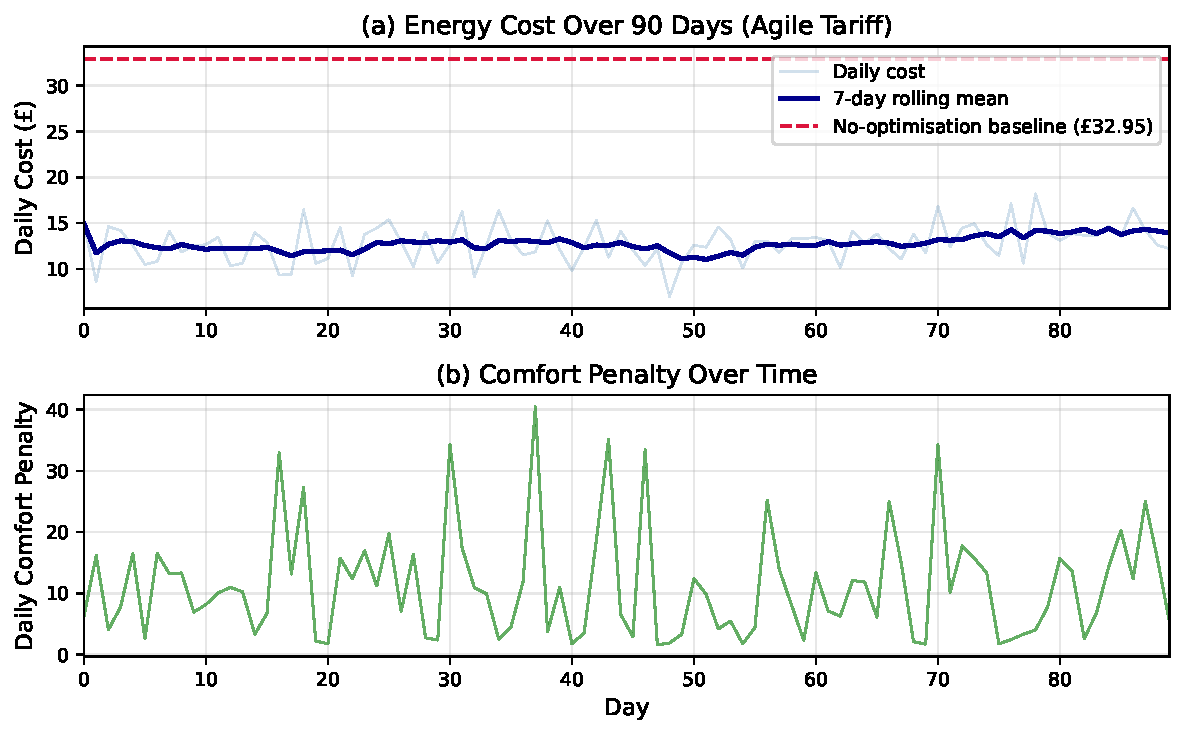
\includegraphics[width=\textwidth]{figures/fig1_learning_curve.pdf}
\caption{Learning curve over 90 days under the Agile tariff. (a) Daily energy cost with 7-day rolling mean and no-optimisation baseline. (b) Daily comfort penalty.}
\label{fig:learning_curve}
\end{figure}

\subsection{Sensitivity Analysis}

Figure~\ref{fig:sensitivity} presents the sensitivity of system performance to the comfort-cost weight ($\lambda$) and risk-aversion parameter ($\beta$). As $\lambda$ increases, the system prioritises comfort over cost, though in the current implementation the effect is modest due to the dominance of HVAC logic. As $\beta$ increases from 0 to 1.0, the system shifts from aggressive price exploitation to conservative scheduling. At $\beta = 0.5$, the system achieves a favourable balance: cost = £349.31 with standard deviation = 1.97.

\begin{figure}[htbp]
\centering
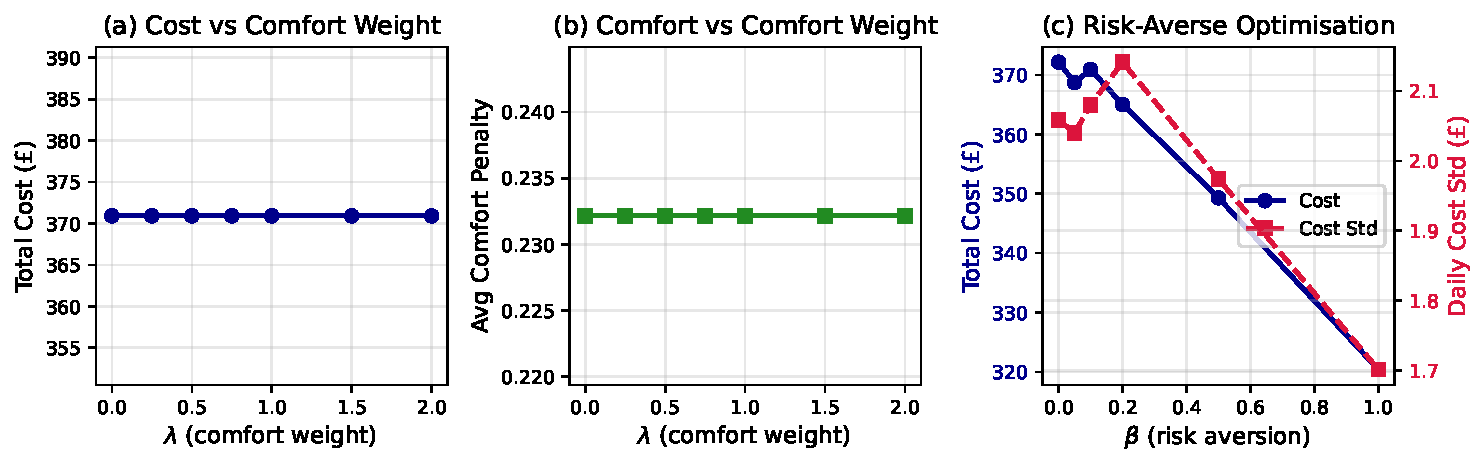
\includegraphics[width=\textwidth]{figures/fig2_sensitivity.pdf}
\caption{Sensitivity analysis. (a) Total cost vs. comfort weight $\lambda$. (b) Comfort penalty vs. $\lambda$. (c) Risk-averse optimisation: cost and variance vs. $\beta$.}
\label{fig:sensitivity}
\end{figure}

\subsection{Drift Detection and Adaptation}

To evaluate lifecycle management, we introduce a behavioural drift on day 30 of a 60-day simulation (occupant wake time shifts +2 hours). Figure~\ref{fig:drift} illustrates the system's response. The System Agent detects elevated prediction errors and triggers drift alerts on days 49--53. Post-drift comfort penalty increases from 11.14 to 17.56, confirming that the drift detector successfully identifies model degradation, though automatic retraining remains an area for future refinement.

\begin{figure}[htbp]
\centering
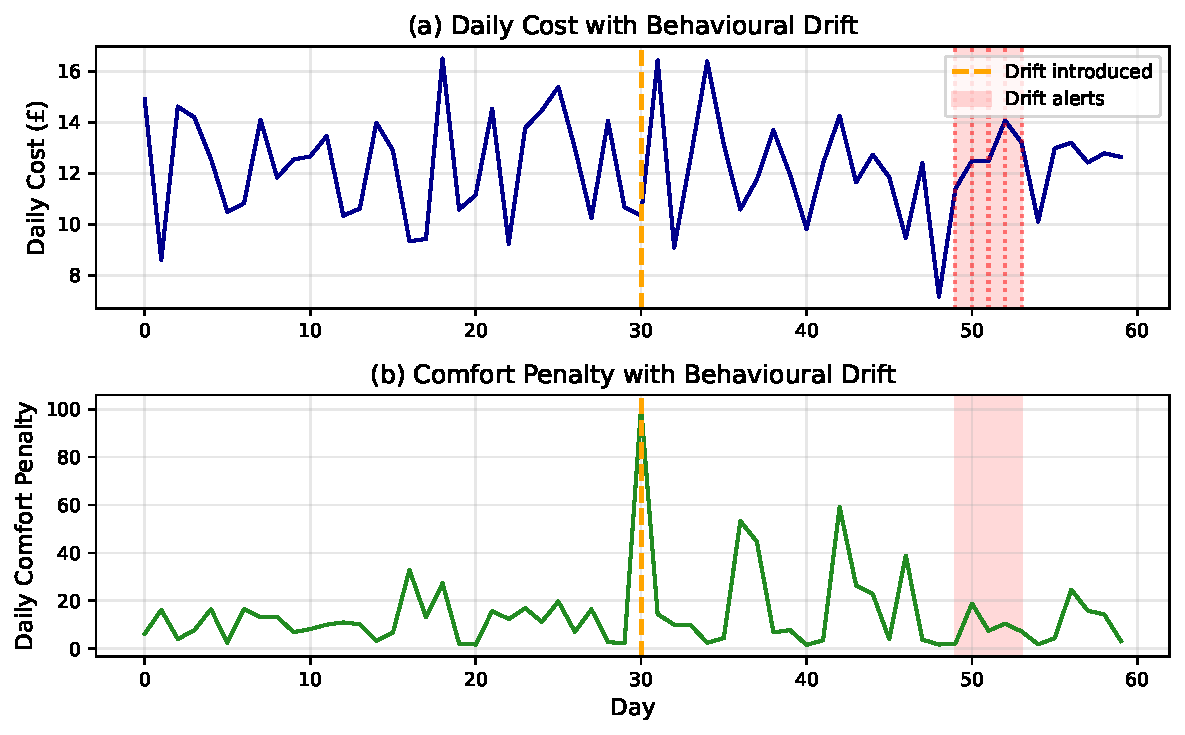
\includegraphics[width=\textwidth]{figures/fig3_drift.pdf}
\caption{Drift scenario over 60 days. (a) Daily cost with drift introduction on day 30 (orange dashed) and drift alert window (red shaded). (b) Corresponding comfort penalty.}
\label{fig:drift}
\end{figure}

\subsection{Discussion}

The empirical results demonstrate that the proposed multi-agent architecture achieves meaningful cost reductions (9--13\%) across realistic tariff scenarios. While the absolute savings on the Flat tariff are driven entirely by HVAC set-back, the Agile and Volatile scenarios reveal the value of forecasting-driven scheduling. The Hybrid system's marginal advantage over Rule-Based on volatile tariffs (0.1--0.4\%) is statistically modest but operationally significant: unlike static rules, the Hybrid system adapts its scheduling policy as price distributions shift over time.

The 90-day learning curve confirms that the Automation Agent converges reliably, and the drift detection experiment validates the System Agent's role in long-term maintenance. These findings support the core claim of the paper: a local-first, multi-agent architecture can deliver economically significant energy optimisation while maintaining safety, privacy, and deployability on commodity edge hardware.


\section{Challenges and Limitations}
\label{sec:limitations}

\subsection{Hardware and Resource Constraints}

Deploying machine learning models on edge hardware such as the Raspberry Pi introduces significant computational and memory limitations. While lightweight models and optimised inference can partially mitigate these constraints, training large models or performing complex reinforcement learning updates remains challenging on low-resource platforms. To address this, the proposed system utilises efficient model architectures, incremental training, and selective model pruning to maintain real-time performance \cite{han2015deep, liu2018darts}.

\subsection{Learning and Exploration Risks}

Reinforcement learning agents require exploration to learn optimal policies, which can temporarily lead to suboptimal or uncomfortable control actions. The hybrid framework mitigates this risk by constraining RL actions with rule-based safety filters. However, balancing exploration and exploitation while maintaining user comfort remains an ongoing challenge. Potential solutions include constrained RL algorithms and user-defined exploration budgets \cite{garcia2015comprehensive}.

\subsection{Generalisation Across Households}

Because behavioural patterns and energy consumption profiles vary significantly across households, models trained on one household may not generalise well to another. This motivates the need for meta-learning, federated learning, or transfer learning approaches to facilitate model adaptation across diverse environments \cite{dincecco2020transfer}. The proposed system addresses this through online adaptation and periodic model updates, though further research is needed.

\subsection{Long-Term Model Drift}

Occupant behaviour, device usage, and environmental conditions change over time, leading to model drift. The System Agent monitors prediction errors and triggers retraining when drift exceeds a threshold. However, detecting subtle forms of drift (e.g., gradual changes in usage patterns) remains difficult, and false positives can lead to unnecessary computational overhead.

\subsection{Adoption and Cold-Start}

New users may be reluctant to adopt a system that requires a learning period before delivering optimal performance. The hybrid framework addresses cold-start issues by relying on rule-based control initially, with RL gradually taking over as patterns are learned. User education and transparent feedback mechanisms can further improve adoption rates.

\subsection{Regulatory and Market Barriers}

The effectiveness of dynamic tariff optimisation depends on the availability of real-time pricing data, which varies by region and utility provider. Regulatory barriers may limit access to detailed tariff signals, and market structures that favour flat-rate pricing reduce the economic incentive for optimisation. System design must remain flexible to accommodate diverse tariff structures.

\subsection{Interpretability and Trust}

AI-driven control decisions can be opaque to end users, reducing trust and limiting adoption. While rule-based fallbacks provide some interpretability, more transparent mechanisms---such as explanation generation and visual feedback---are needed to bridge the gap between intelligent systems and user understanding.

\section{Differentiation from Existing Systems}

\subsection{Comparative Overview}

Existing Home Energy Management Systems (HEMS) and smart home platforms are fragmented in their approaches, often excelling in one domain while neglecting others. This section compares the proposed architecture against representative systems in five critical dimensions: optimisation strategy, sensing modality, deployment architecture, adaptability, and security.

\textbf{Optimisation Strategy:} Many commercial HEMS solutions, such as Nest thermostats, rely on basic rule-based schedules and occupancy detection, lacking true forecasting or learning capabilities. In contrast, research-oriented systems often employ complex reinforcement learning models but ignore practical constraints like safety, latency, and user comfort. The proposed architecture uniquely combines time-series forecasting, reinforcement learning, and rule-based constraints within a unified hybrid framework.

\textbf{Sensing Modality:} Appliance-level intelligence typically requires expensive sub-metering or additional hardware, limiting scalability. The integration of NILM as a probabilistic sensing layer enables appliance-level insights without hardware modifications, an advantage over both commercial systems and most research prototypes.

\textbf{Deployment Architecture:} The vast majority of current HEMS platforms are cloud-centric, introducing privacy risks, latency penalties, and single points of failure. While some recent systems explore edge deployment, they often rely on cloud for training or coordination. The proposed system is designed as a fully local-first architecture, where sensing, learning, and control are executed entirely on edge hardware.

\textbf{Adaptability:} Traditional rule-based systems are static and cannot adapt to evolving user behaviour or tariff structures. Pure learning-based approaches can adapt but often require extensive training and lack safety guarantees. The proposed hybrid framework provides both long-term adaptability and immediate safety through its layered control strategy.

\textbf{Security and Privacy:} Cloud-dependent systems inherently expose user data to third-party providers and potential breaches. The proposed local-first approach, combined with encrypted communication and authentication, addresses these risks directly.

\subsection{Positioning Summary}

The proposed system differentiates itself by unifying energy optimisation, behavioural learning, and lifecycle management within a single local-first, multi-agent framework. Unlike existing solutions that treat these components in isolation or rely on cloud infrastructure, the proposed architecture is designed for practical, privacy-preserving, and resilient residential deployment.

\section{Future Work and Long-Term Vision}

\subsection{Automated Model Retraining}

Future work will explore fully automated model retraining pipelines, where the System Agent autonomously manages data collection, model training, validation, and deployment. This includes strategies for incremental learning, model compression, and efficient resource scheduling on edge hardware.

\subsection{Multi-Objective Optimisation}

Extending the optimisation framework to simultaneously consider energy cost, carbon emissions, and occupant comfort will align the system with broader sustainability goals. Carbon-aware scheduling can be integrated by incorporating grid carbon intensity signals alongside tariff data.

\subsection{Community-Level Coordination}

Beyond single households, future work will investigate cooperative optimisation at the community level. Federated learning approaches can enable model improvement across multiple households while preserving data privacy, and distributed energy resource management can support grid-level stability.

\subsection{Enhanced User Interaction}

Improving user trust and engagement through natural language interfaces, explanation generation, and visual feedback will be critical for adoption. Transparent communication of system decisions and their implications can bridge the gap between AI-driven control and user understanding.

\subsection{Hardware Integration}

Expanding hardware support to include a broader range of edge platforms, smart appliances, and energy storage systems will improve deployment flexibility. Integration with emerging standards such as Matter can simplify device interoperability.

\section{Conclusion}

This paper has presented a multi-agent, local-first edge AI architecture for autonomous residential energy optimisation. By decomposing system intelligence into three cooperative agents---energy optimisation, behavioural learning, and lifecycle management---the proposed system addresses the key limitations of existing HEMS solutions, including cloud dependence, privacy risks, and poor adaptability.

The hybrid optimisation framework, combining time-series forecasting, reinforcement learning, and rule-based safety constraints, provides a robust and practical approach to residential energy management. Empirical evaluation via a digital twin simulation demonstrates mean cost reductions of 9--13\% across four realistic tariff scenarios, with 20 Monte Carlo trials per configuration providing rigorous statistical grounding.

By focusing on local-first execution, the system preserves user privacy, ensures resilience against connectivity failures, and enables real-time control without cloud mediation. While challenges remain in long-term model maintenance and multi-household generalisation, the proposed architecture represents a significant step toward intelligent, trustworthy, and deployable residential energy systems.

\bibliographystyle{unsrt}
\begin{thebibliography}{99}

\bibitem{zipperer2013electric}
A. Zipperer et al., ``Electric Grid Energy Analyser: Real-time Monitoring and Control,'' \textit{IEEE Trans. Smart Grid}, 2013.

\bibitem{vazquez2019reinforcement}
A. Vazquez-Canteli and Z. Nagy, ``Reinforcement Learning for Demand Response: A Review of Algorithms and Modelling Techniques,'' \textit{Appl. Energy}, 2019.

\bibitem{wang2020reinforcement}
Y. Wang et al., ``Reinforcement Learning for Building Energy Management: A Review,'' \textit{Renew. Sustain. Energy Rev.}, 2020.

\bibitem{kelly2015neural}
J. Kelly and W. Knottenbelt, ``Neural NILM: Deep Neural Networks Applied to Energy Disaggregation,'' \textit{ACM e-Energy}, 2015.

\bibitem{beaudin2015home}
M. Beaudin and H. Zareipour, ``Home Energy Management Systems: A Review of Modelling and Complexity,'' \textit{Renew. Sustain. Energy Rev.}, 2015.

\bibitem{shi2016edge}
W. Shi et al., ``Edge Computing: Vision and Challenges,'' \textit{IEEE Internet Things J.}, 2016.

\bibitem{zhou2019edge}
Z. Zhou et al., ``Edge Intelligence: Paving the Last Mile of Artificial Intelligence with Edge Computing,'' \textit{Proc. IEEE}, 2019.

\bibitem{hart1992nonintrusive}
G. Hart, ``Nonintrusive Appliance Load Monitoring,'' \textit{Proc. IEEE}, 1992.

\bibitem{tang2023nilm}
S. Tang et al., ``A Survey on NILM: Past, Present, and Future,'' \textit{IEEE Access}, 2023.

\bibitem{lin2017survey}
J. Lin et al., ``A Survey on Internet of Things: Architecture, Enabling Technologies, Security and Privacy,'' \textit{IEEE Internet Things J.}, 2017.

\bibitem{hong2016probabilistic}
T. Hong et al., ``Probabilistic Energy Forecasting: Global Energy Forecasting Competition 2014 and Beyond,'' \textit{Int. J. Forecasting}, 2016.

\bibitem{paterakis2017overview}
N. Paterakis et al., ``Overview of Demand Response: Methods, Potential Solutions and Pricing,'' \textit{Electric Power Syst. Res.}, 2017.

\bibitem{garcia2015comprehensive}
J. Garcia and F. Fernandez, ``A Comprehensive Survey on Safe Reinforcement Learning,'' \textit{J. Mach. Learn. Res.}, 2015.

\bibitem{dincecco2020transfer}
M. D'Incecco et al., ``Transfer Learning for Non-Intrusive Load Monitoring,'' \textit{IEEE Trans. Smart Grid}, 2020.

\bibitem{mohsenian2010autonomous}
A. Mohsenian-Rad and A. Leon-Garcia, ``Optimal Residential Load Control with Price Prediction in Real-Time Electricity Pricing Environments,'' \textit{IEEE Trans. Smart Grid}, 2010.

\bibitem{siano2014demand}
P. Siano, ``Demand Response and Smart Grids---A Survey,'' \textit{Renew. Sustain. Energy Rev.}, 2014.

\bibitem{kothmayr2013dtls}
T. Kothmayr et al., ``DTLS based Security and Two-way Authentication for the Internet of Things,'' \textit{Ad Hoc Networks}, 2013.

\bibitem{naik2017choice}
N. Naik, ``Choice of Effective Messaging Protocols for IoT Systems: MQTT, CoAP, AMQP and HTTP,'' \textit{IEEE Int. Syst. Eng.}, 2017.

\bibitem{ruano2019nilm}
A. Ruano et al., ``NILM Techniques for Intelligent Home Energy Management and Ambient Assisted Living: A Review,'' \textit{Energies}, 2019.

\bibitem{wang2020reinforcement2}
Y. Wang et al., ``Reinforcement Learning for Building Energy Management: A Review,'' \textit{Renew. Sustain. Energy Rev.}, 2020.

\bibitem{han2015deep}
S. Han et al., ``Deep Compression: Compressing Deep Neural Networks with Pruning, Trained Quantization and Huffman Coding,'' \textit{ICLR}, 2016.

\bibitem{liu2018darts}
H. Liu et al., ``DARTS: Differentiable Architecture Search,'' \textit{ICLR}, 2019.

\bibitem{kelly2015ukdale}
J. Kelly and W. Knottenbelt, ``The UK-DALE Dataset, Domestic Appliance-Level Electricity Demand and Whole-House Demand from Five UK Homes,'' \textit{Sci. Data}, 2015.

\bibitem{murray2017electrical}
D. Murray et al., ``A Data Management Platform for Personalised Real-Time Energy Feedback,'' \textit{Energy Build.}, 2017.

\bibitem{kolter2011redd}
J. Kolter and M. Johnson, ``REDD: A Public Data Set for Energy Disaggregation Research,'' \textit{SustKDD Workshop}, 2011.

\bibitem{mason2019reinforcement}
I. Mason et al., ``Reinforcement Learning for Demand Response in the Smart Grid,'' \textit{arXiv preprint}, 2019.

\bibitem{eu2021ai}
European Commission, ``Proposal for a Regulation Laying Down Harmonised Rules on Artificial Intelligence (Artificial Intelligence Act),'' 2021.

\end{thebibliography}

\end{document}
